% !TeX root = ../main-english.tex
% !TeX spellcheck = en-US
% !TeX encoding = utf8
% -*- coding:utf-8 mod:LaTeX -*-

%This smart spell only works if no changes have been made to the chapter
%using the options proposed in preambel/chapterheads.tex.
\setchapterpreamble[u]{%
	\dictum[Albert Einstein]{If we knew what it was we were doing, it would not be called research, would it?}
}

\chapter{Reproducible state space modeling}
\label{k5}

Look mom, some text!

\section{Shared response modeling}
\pagebreak

\section{Simulation study}
\pagebreak

\section{The MEMENTO study}

%Rationale from Luka
In natural settings, value-based decisions under risk often have to be made without visual presence of competing alternatives.
Therefore, the subjective value of alternative options has to be held in working memory in order to form a categorical choice.
Numerous studies report neuronal signals representing value.
However, the temporal dynamics of the decision process as well as the maintenance of different valued options in working memory are less thoroughly investigated questions.
Therefore, the memento study investigated how decision-relevant information is retained in working memory using a decision making task with concurrent \gls{meg} acquisition.
It was acquired as part of the SFB 779 project B16N (``offline value representations in sequential decision making'') at the Otto-von-Guericke University Magdeburg in 2016 by \citet{kaiser}, and has not been previously published.
The following study overview adheres to the COBIDAS MEEG reporting guidelines for reproducible MEEG research \citep{pernet2020issues}.
The code used for preprocessing and analysis was bundled into a publicly available Python package \texttt{pymento\_meg} and is available from GitHub\footnote{\url{https://github.com/adswa/pymento_meg}} and \url{PyPi.org}.
Underlying software packages are listed in Table TODO.

\subsection{Participants}

$N = 22$ right-handed, healthy participants with normal or corrected-to-normal vision were recruited at the Center for Behavioral Brain Sciences and on the university campus Magdeburg.
Their mean age was 26 years, and 10 participants were male.
Handedness was assessed with the Edinburgh Handedness Inventory \citep{oldfield1971assessment}.
Participants gave their informed consent to participate in the study, and received a base monetary compensation in the order of 8€ per hour with a performance-dependent bonus of up to 3€.
Ethics approval was obtained from the University Clinic Magdeburg.

\subsection{Experimental design}

The experiment consisted of 510 trials, grouped into 5 blocks with a variable break in between.
Each trial required a decision between one of two stimulus options, presented as gabor patches on the left and right side of the screen (\cref{fig:memento_trial}).
Importantly, stimulus options were presented in succession, with a delay period through which the decision-relevant properties of the first stimulus had to be retained in working memory.
The number of stripes in the gabor patch encoded the reward magnitude (either 0.5, 1, 2, or 4 points), and the angle of stripes encoded reward probability (either 10\%, 20\%, 40\%, or 80\%): The more stripes, the higher the reward, and the larger the angle, the higher the probability. \cref{fig:memento_stim} provides an overview.
Participants learned these associations in a tutorial prior to the experiment (\cref{fig:memento_tutorial}).
Each trial started with a fixation cross (1000-1900ms, jittered), followed by the first stimulus on the left side of the screen for 700ms, a 2000ms delay period through which the phrase ``or'' was presented in the center of the screen, the second stimulus option on the right side of the screen for 700ms, and a feedback screen.
Once the second stimulus option was displayed, participants chose the left or right option via a button press with the right or left index finger, respectively.
The feedback screen showed both options side by side with a frame around the chosen option, and revealed which option had been rewarded via color coding (red: unrewarded, green: rewarded).
If a decision was not made within 5 seconds, the trial was aborted and participants saw a message to respond faster.
A progress bar at the bottom of the screen tracked gains over time, resulting in a bonus payment whenever it hit a gold target line.
Participants were instructed to maximize their gains and to respond as fast as possible.
Stimulus presentation was controlled by Psychtoolbox \citep{kleiner2007s} running on Matlab 2012b (The Mathworks Company, Natick, MA).
All stimuli were presented on a grey background with a contrast optimized for the MEG recording chamber.
A photodiode, taped onto the stimulation screen, was used to determine visual stimulus onsets.
TODO: Add delay
In total, the experiment lasted approximately 60 minutes.

\begin{figure}
	\centering
	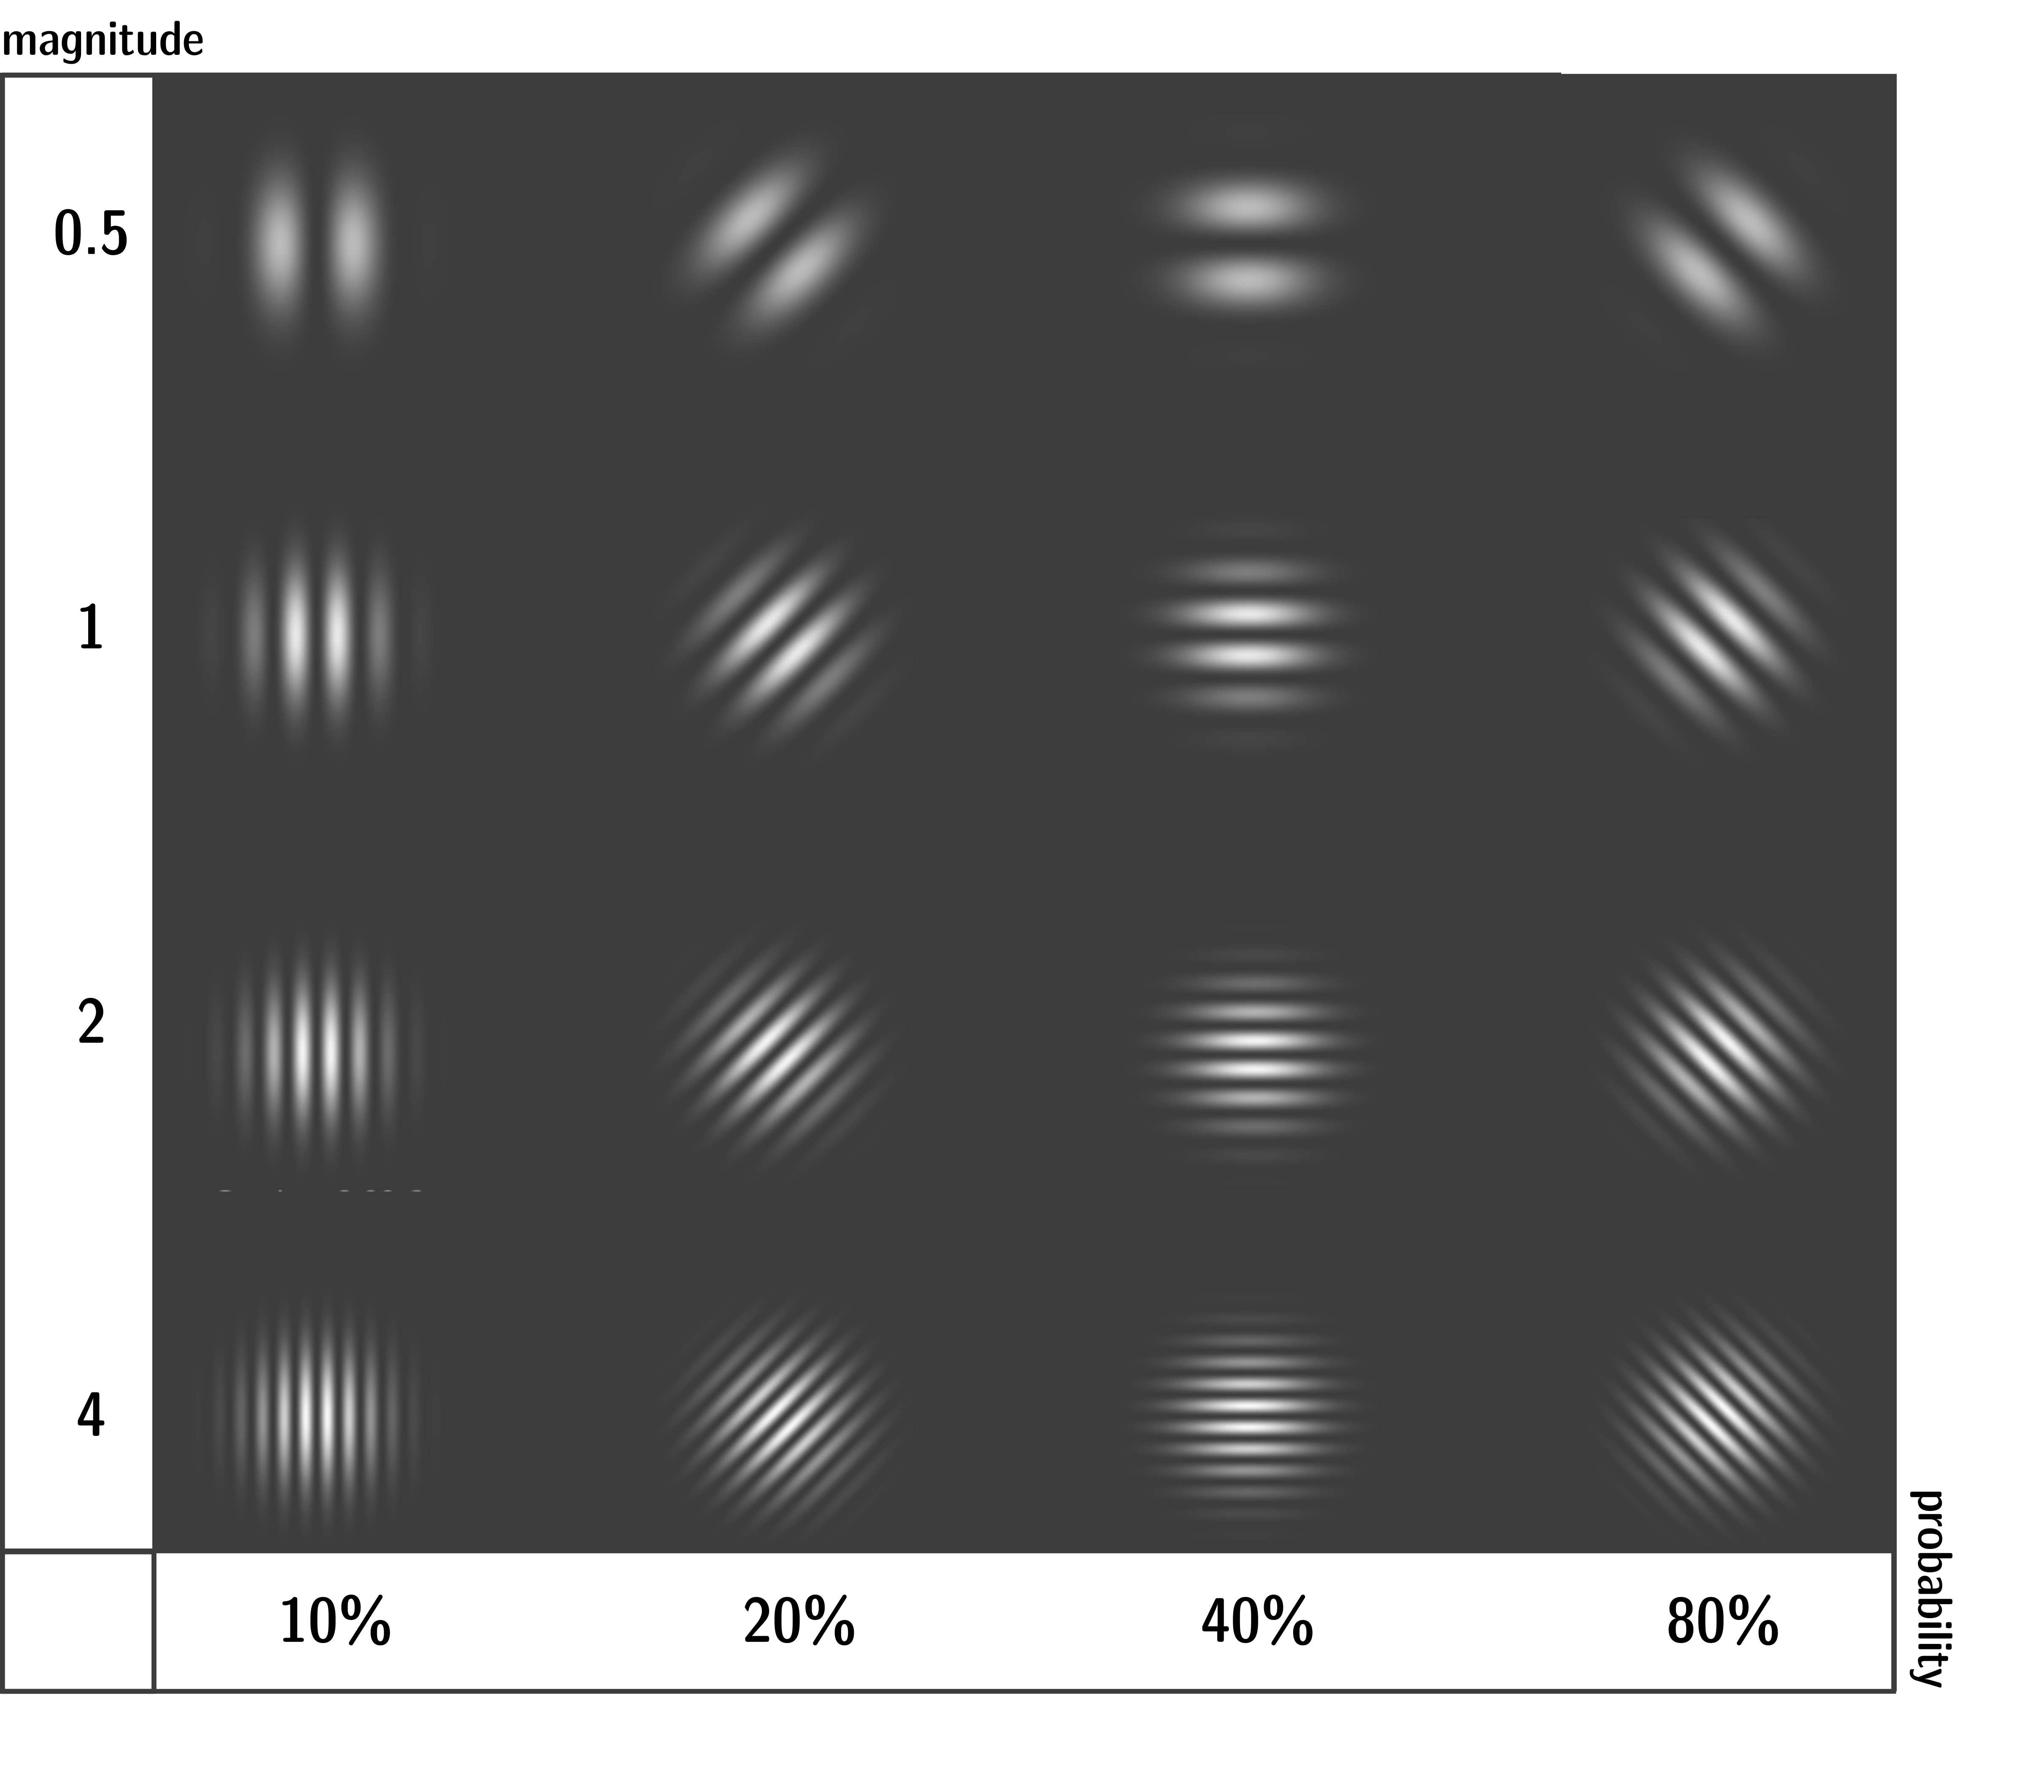
\includegraphics[width=0.5\textwidth]{memento/memento_stimuli.png}
	\caption[Stimulus overview]{Stimulus overview: Gabor patches varied in the number of stripes and their angle, encoding magnitude and probability, respectively.}
	\label{fig:memento_stim}
\end{figure}

\begin{figure}
	\begin{subfigure}{.54\textwidth}
	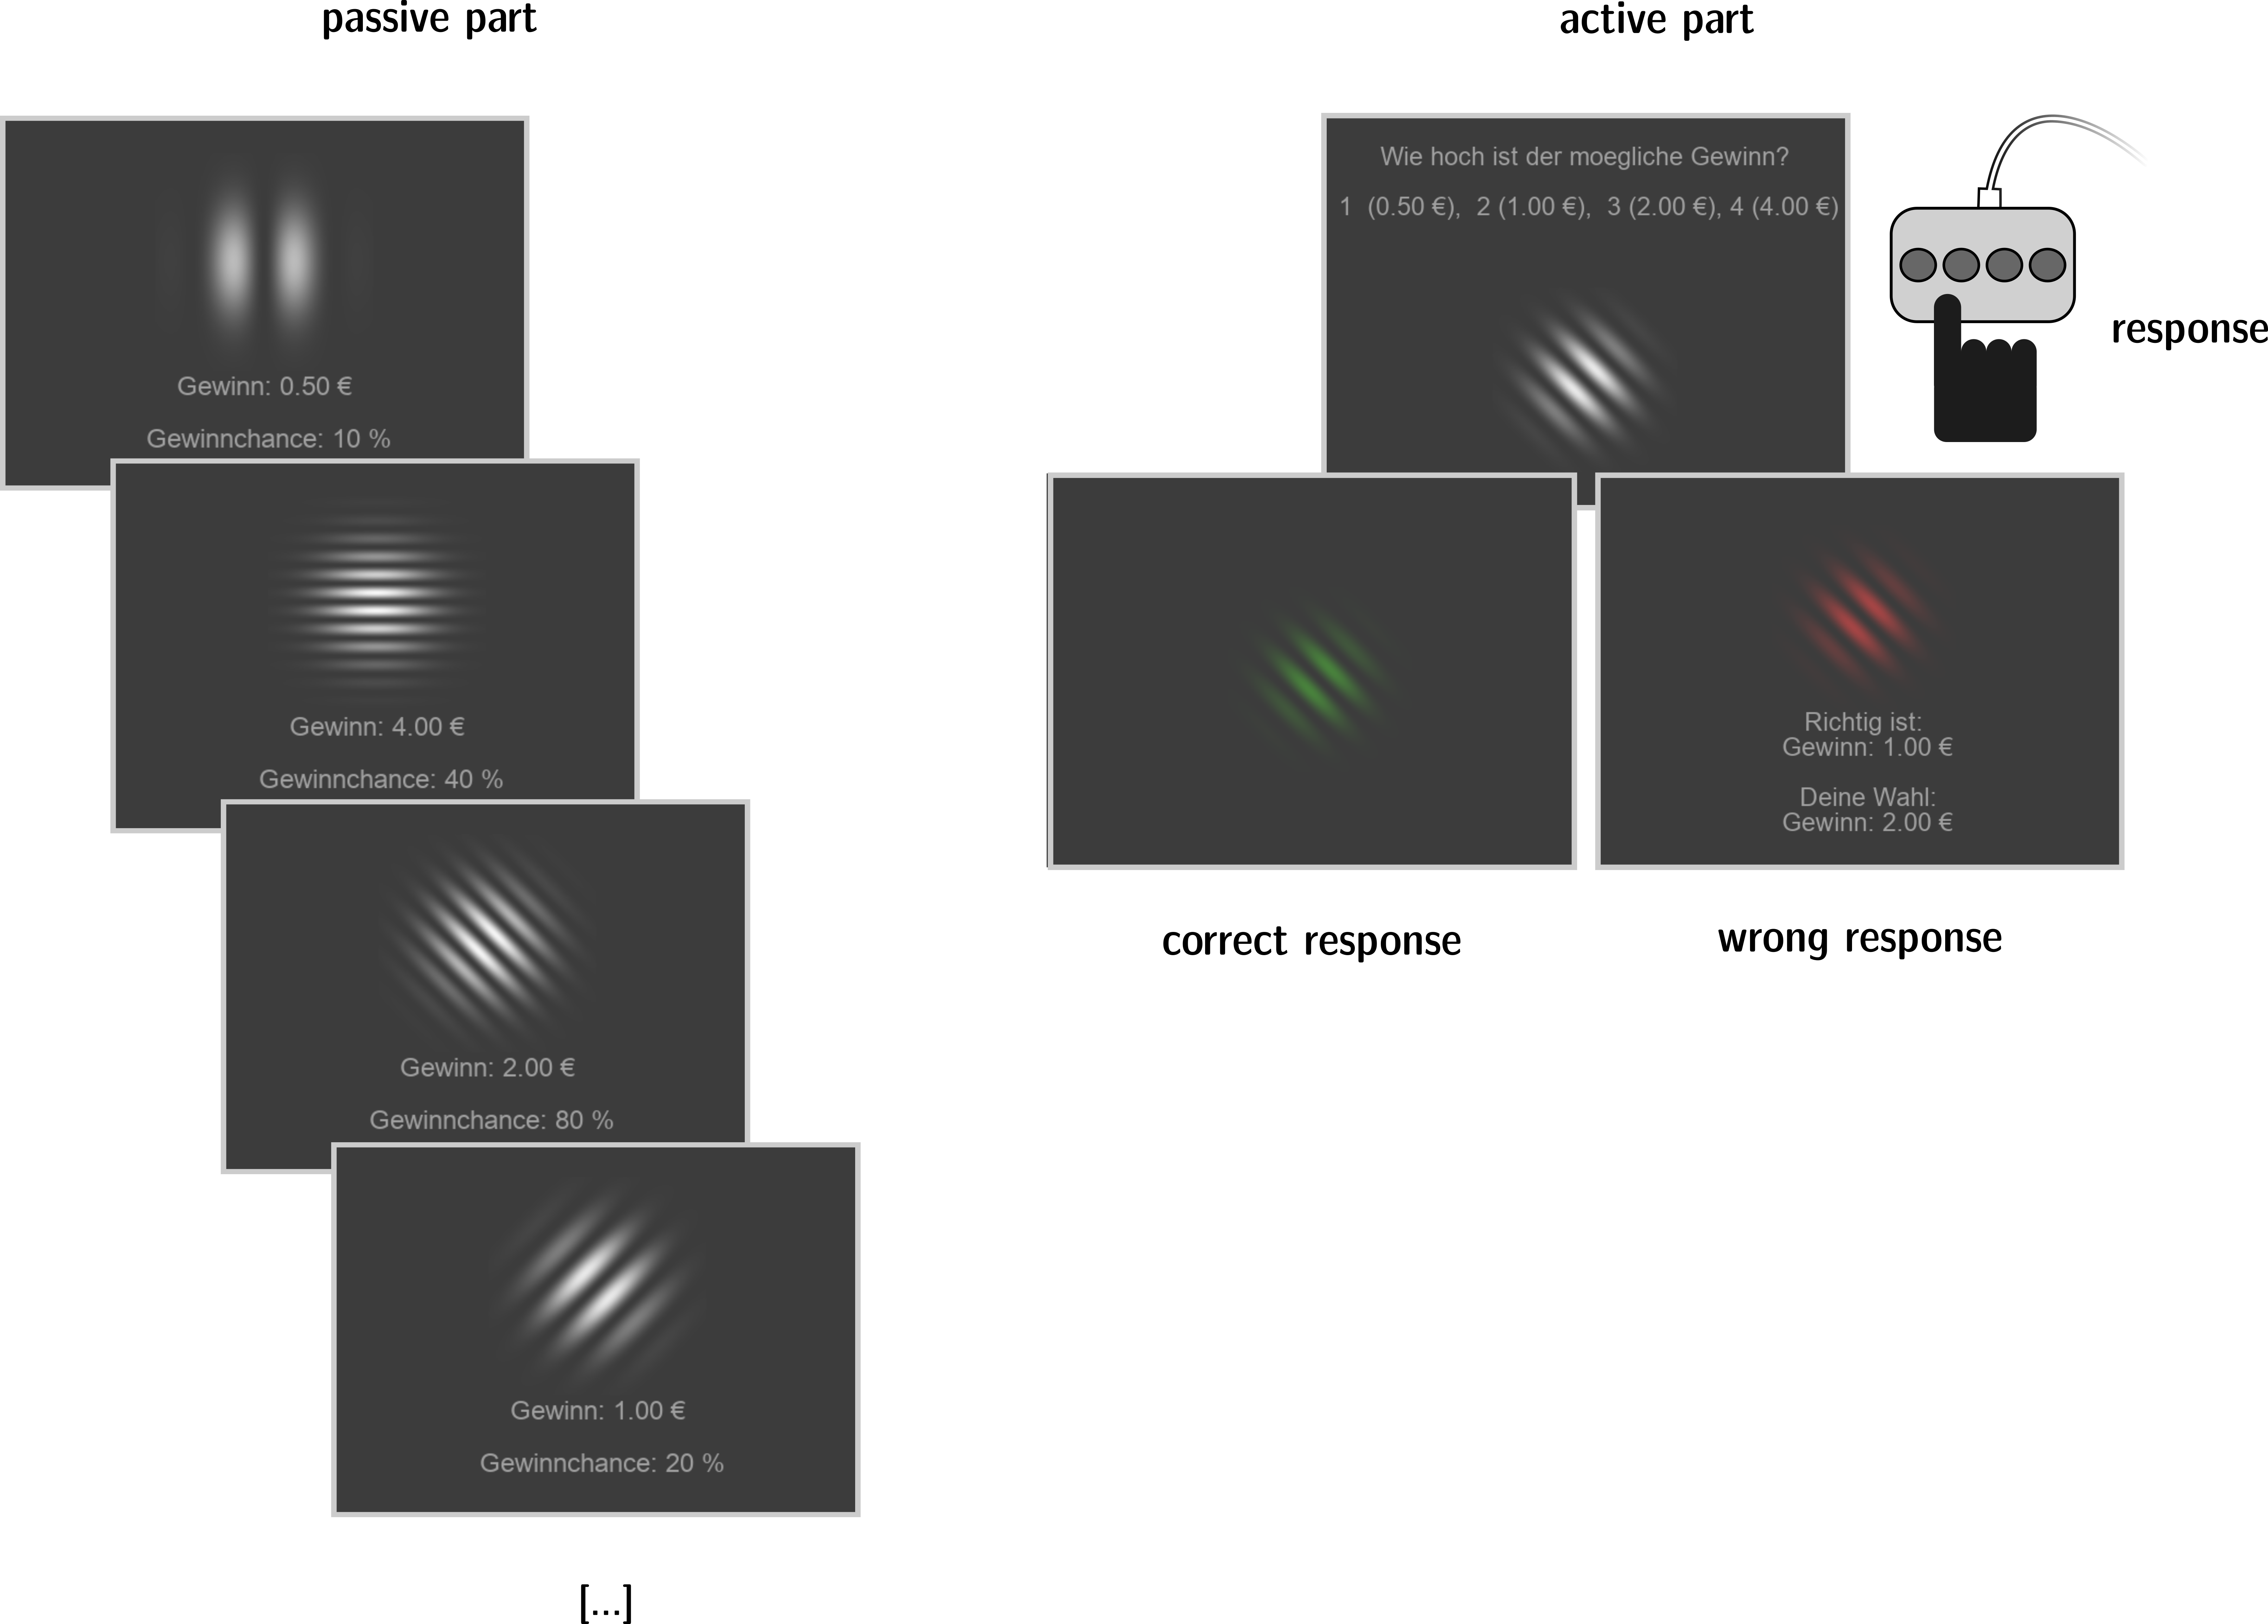
\includegraphics[width=\textwidth]{memento/memento_tutorial.png}
	\caption{Schematic overview of the tutorial.}
	\label{fig:memento_tutorial}
	\end{subfigure}
	\begin{subfigure}{.45\textwidth}
	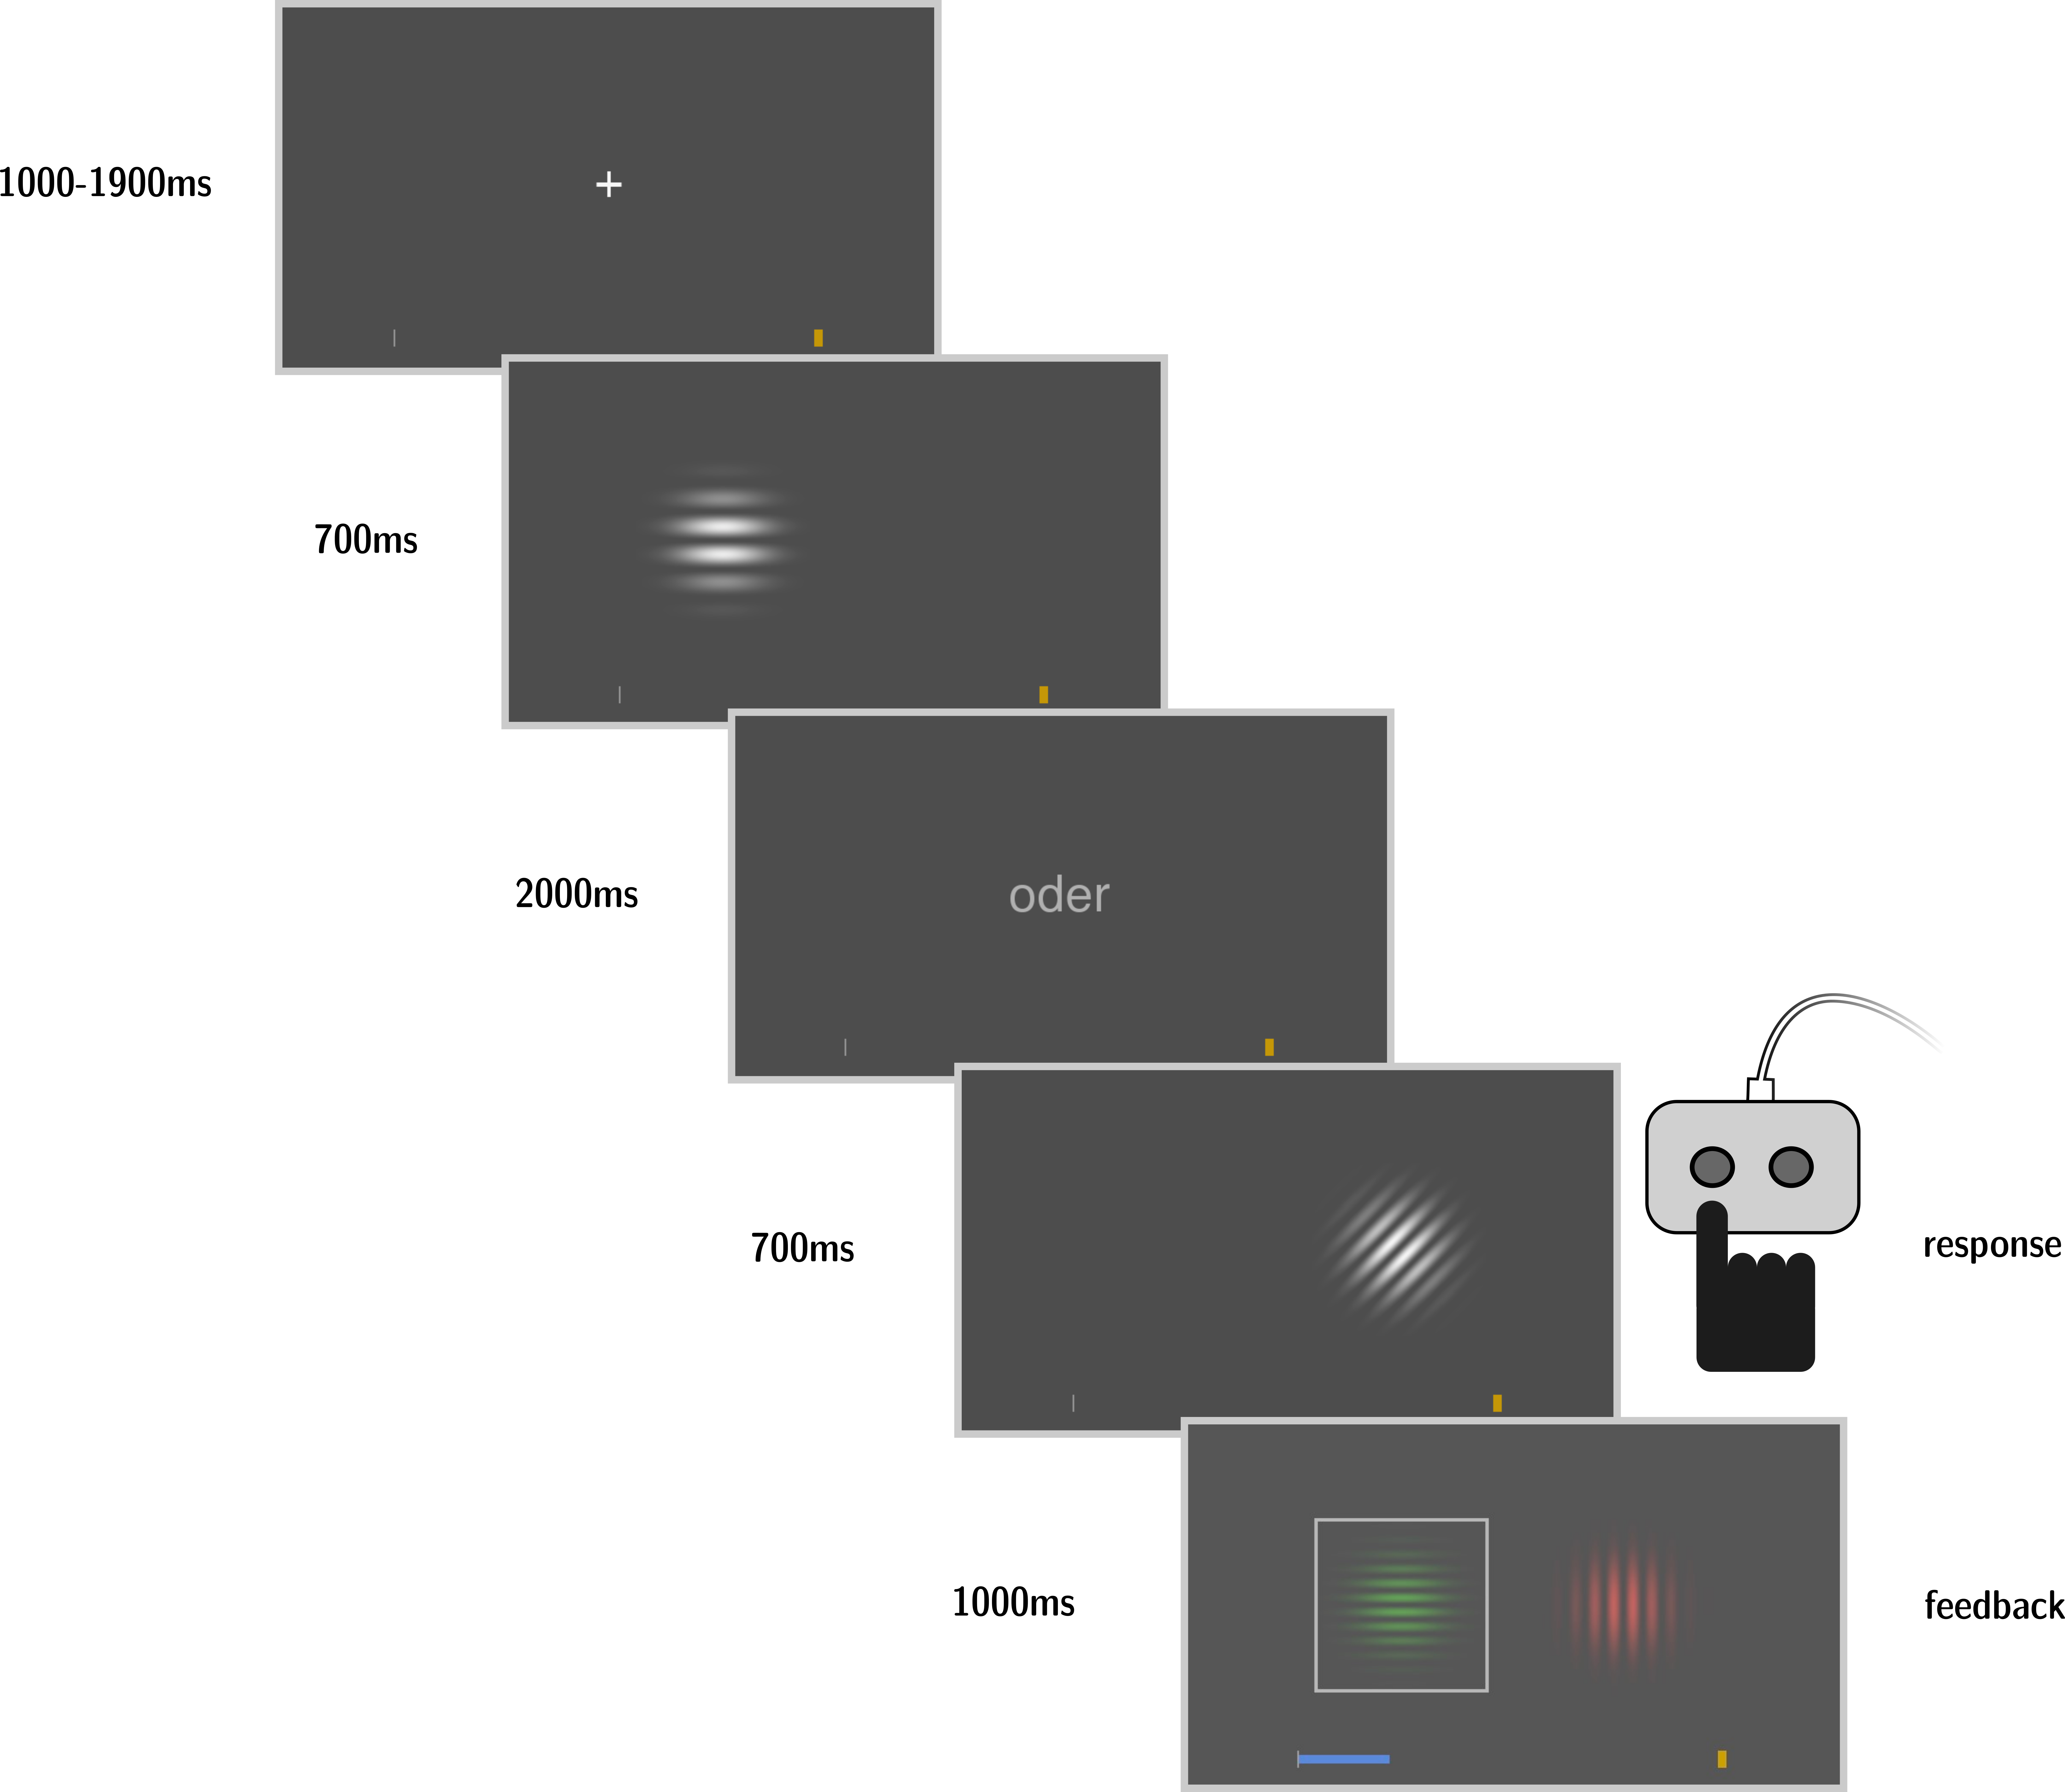
\includegraphics[width=\textwidth]{memento/memento_experiment.png}
	\caption{Schematic overview of a single trial.}
	\label{fig:memento_trial}
\end{subfigure}
	\caption[Memento: Tutorial and trial overview]{Schematic overview of the tutorial (\ref{fig:memento_tutorial}) and a single trial in the experiment (\ref{fig:memento_trial}).
	The tutorial was split in an active and a passive part.
	In the passive part, participants were presented with a stimulus and how its properties translated to reward magnitude and probability. All possible magnitude and probability combinations were presented twice, and participants controlled the pace. The active part then tested participants' knowledge by presenting with a stimulus without the annotation. Based on a text prompt, participants had to report its associated magnitude or probability via button press. They received feedback with a green colored stimulus for a correct response, or, for an incorrect response, a red colored stimulus together with a report of their response versus the true response.
	}
\label{fig:memento}
\end{figure}


\subsection{MEG acquisition}

Following a metal test, MEG data were acquired on an Elekta Neuromag TRIUX System with internal helium recycler and 306 sensors (204 planar gradiometers and 102 magnetometers) in a magnetically shielded room.
Participants were instructed to take a comfortable seating position and sit as still as possible.
The experiment was presented on a screen in a distance of one meter from the sitting participants via a projector with a refresh rate of 75 Hz located outside the MEG recording chamber.
Additional sensors captured confounding biological signals:
Lateral and vertical eye movements and blinks were captured using electrooculography surface electrodes on the tori supra- and infraorbitalis and next to the external canthi.
Heartbeat artifacts were recorded with an electrocardiogram.
Head position indicator coils captured the participants head movements.
Behavioral responses were registered using an MEG compatible keyboard.
The neural data was recorded at a sampling rate of 1000Hz and active internal shielding (IAS).


\subsection{Preprocessing}

Prior to preprocessing, raw data were restructured to \gls{BIDS} format (v1.4.0) using mne-bids \citep{Appelhoff2019}.
Simultaneously, behavioral log files were transformed from proprietary .mat into the TSV format.

As the first step of preprocessing, the spatiotemporal extension of the \gls{SSS} method \citep{taulu2005presentation}, \textit{\gls{tSSS}} \citep{taulu2006spatiotemporal}, was applied, as is common for recordings on Neuromag MEG systems with active internal shielding.
\gls{SSS} and \gls{tSSS} remove strong interference from external noise sources and sources within the body itself from the MEG signal.
The methods can be applied on whole-scalp multichannel data when the precise sensor calibrations are known, and were initially developed as the proprietary MaxFilter\textsuperscript{TM} algorithm by Elekta Neuromag.
To this end, Neuromag systems provide a cross-talk compensation and fine calibration file which reduces interference between their co-located magnetometer and paired gradiometer sensor units and encodes site-specific information about sensor orientation and calibration, respectively.
\gls{SSS} decomposes \gls{meg} signals into elementary magnetic fields from sources within the sensor helmet (the \textit{internal} subspace) and into a set for fields arising from sources outside (the \textit{external} subspace) based on the Maxwell equations \citep{taulu2006spatiotemporal}.
As the internal and external subspaces are provably linearly independent, brain signals are then reconstructed by retaining only sources inside the helmet, thus excluding external inferences.
According to \citet{taulu2006spatiotemporal}, \gls{SSS} can separate brain signals from sources >0.5m away, suppressing external interference by a factor >100.
The spatiotemporal extension \gls{tSSS} can further detect inferences from closer sources such as stimulators or pacemakers.
These are estimated based on the fact that their strength typically exceeds that of sensor noise and they thus, unlike brain signal, leak into both the internal and external part of the \gls{SSS} reconstruction.
After detecting components with a high temporal correlation between the external and internal subspaces, \gls{tSSS} removes close-by artifacts by projecting the components common to the internal and external subspace out of the internal subspace.
In the absence of nearby artifacts, \gls{tSSS} reduces to \gls{SSS} \citep{taulu2009removal}.
\gls{tSSS} was implemented using mne-python's open source implementation \texttt{maxwell\_filter()} with a chunk duration of 10 seconds and a correlation threshold of at least $0.98$.
Prior to \gls{tSSS}, bad channels were detected and annotated automatically in order to prevent bad channel noise from spreading.
To compensate for head movements, measurements from the head position indicator coils were used to estimate subject motion, and motion correction was then performed as part of the \gls{tSSS} procedure.
After \gls{tSSS}, gradiometers and magnetometers contain highly similar information and have an altered inter-channel correlation structure because they were reconstructed from a common 80-dimensional subspace \citep{jas2018reproducible}.
In all following analyses, these channels are thus treated as a single sensor type.
Formerly bad channels have also been effectively repaired by the procedure.
After \gls{tSSS}, some spectral artifacts remained in the data, among them power line noise at 50Hz and a spectral peak at 60Hz, likely originating from the presentation screen's refresh rate.
ZAPline filtering \citep{de2020zapline} was performed to remove them using \texttt{meegkit} \citep{barascud2022}.
Figures \ref{fig:prezap} and \ref{fig:postzap} show power spectral density plots of the signal pre and post (effective window size: 2.048 s) applying ZAPline filters.


\begin{figure}
	\begin{subfigure}{.49\textwidth}
		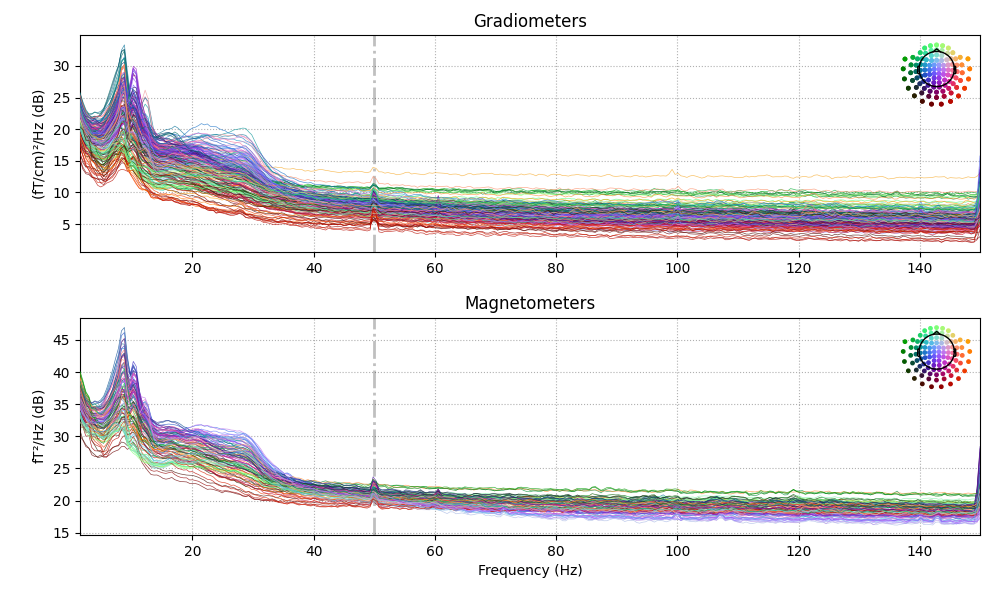
\includegraphics[width=\textwidth]{memento/psd_pre_zapline.png}
		\caption{Power spectral density before ZAPline filtering}
		\label{fig:prezap}
	\end{subfigure}
	\begin{subfigure}{.49\textwidth}
		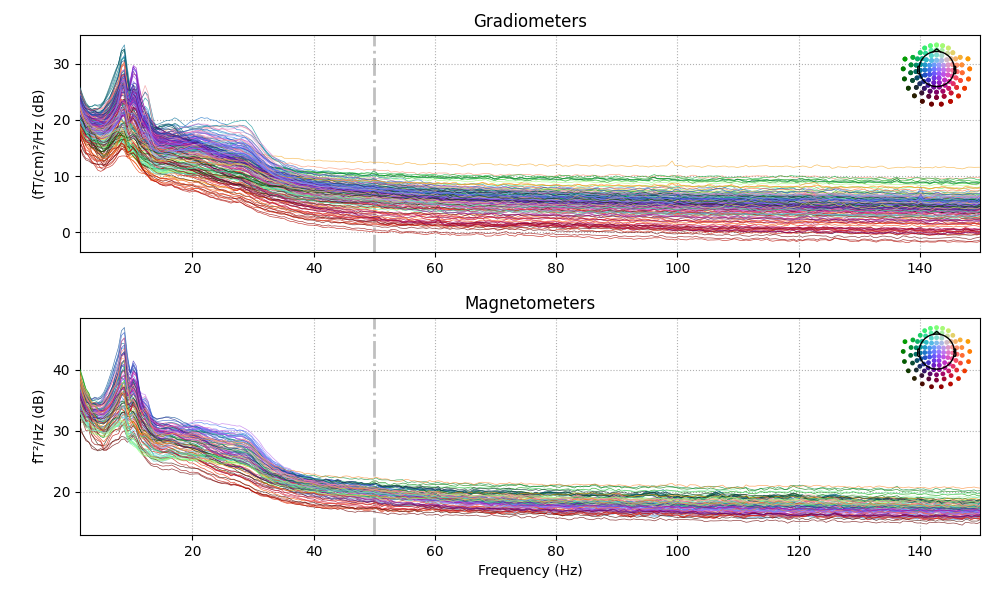
\includegraphics[width=\textwidth]{memento/psd_post_zapline.png}
		\caption{Power spectral density after ZAPline filtering}
		\label{fig:postzap}
	\end{subfigure}
	\caption[Power spectral density before and after ZAPLine filtering]{Power spectral density of all MEG channels
		from a single subject before (\ref{fig:prezap}) and after (\ref{fig:postzap}) ZAPLine filtering.
		Two spikes at 50Hz (power-line frequency) and 60Hz (likely an artifact of the stimulus presentation) are markedly reduced afterwards.
	}
	\label{fig:zapline_psd}
\end{figure}

Next, data were first low-pass filtered with a 100Hz lowpass FIR filter to constrain it into a frequency range of interest.
The filter properties are reported in \ref{fig:preproc} and a visualization is in \ref{fig:filter}.
As eye movements, eye blinks, heart beats, and facial muscle contractions survive \gls{tSSS}, \gls{ica} was used to detect and remove these artifacts.
% The slow drifts are problematic because they reduce the independence of the assumed-to-be-independent sources (e.g., during a slow upward drift, the neural, heartbeat, blink, and other muscular sources will all tend to have higher values), making it harder for the algorithm to find an accurate solution. A high-pass filter with 1 Hz cutoff frequency is recommended. However, because filtering is a linear operation, the ICA solution found from the filtered signal can be applied to the unfiltered signal https://ieeexplore.ieee.org/document/7319296/
As ICA is sensitive to low-frequency drifts \citep{winkler2015ICA}, the data were first processed with a temporary one-pass, zero-phase, non-causal highpass filter (firwin method, Hamming window with 0.0194 passband ripple and 53 dB stopband attenuation, a lower passband edge of 1.00, lower transition bandwidth of 1.00 Hz (-6 dB cutoff frequency: 0.50 Hz), and a filter length of 3301 samples (3.301 s)).
As ICA can further be sensitive to bad segments in the recording, data were temporarily epoched into 5 second splits from the onset of the fixation cross.
\texttt{autoreject} was then used on the first 200 of these epochs to estimate the noise level and compute rejection thresholds.
Afterwards, FastICA \citep{hyvarinen1999fast} was used to decompose the signal into 45 independent components.
For most subjects, components corresponding to ECG activity were identified using cross-trial phase statistics \citep{dammers2008integration} with an automatically computed threshold of 0.16 for the Kuiper statistic, and EOG related components were found using Pearson correlation.
For one subject, however, the ECG channel was flat, and components were manually selected.
Afterwards, the ICA solution was applied to the continuous recording and detected ECG and EOG components were zeroed out.

As a final step, the continous recording was chunked into Epochs, and autoreject was used to detect and repair or drop bad epochs.
Figure \ref{fig:preproc} summarizes the preprocessing steps.



\begin{figure}
	\begin{subfigure}{0.4\textwidth}
		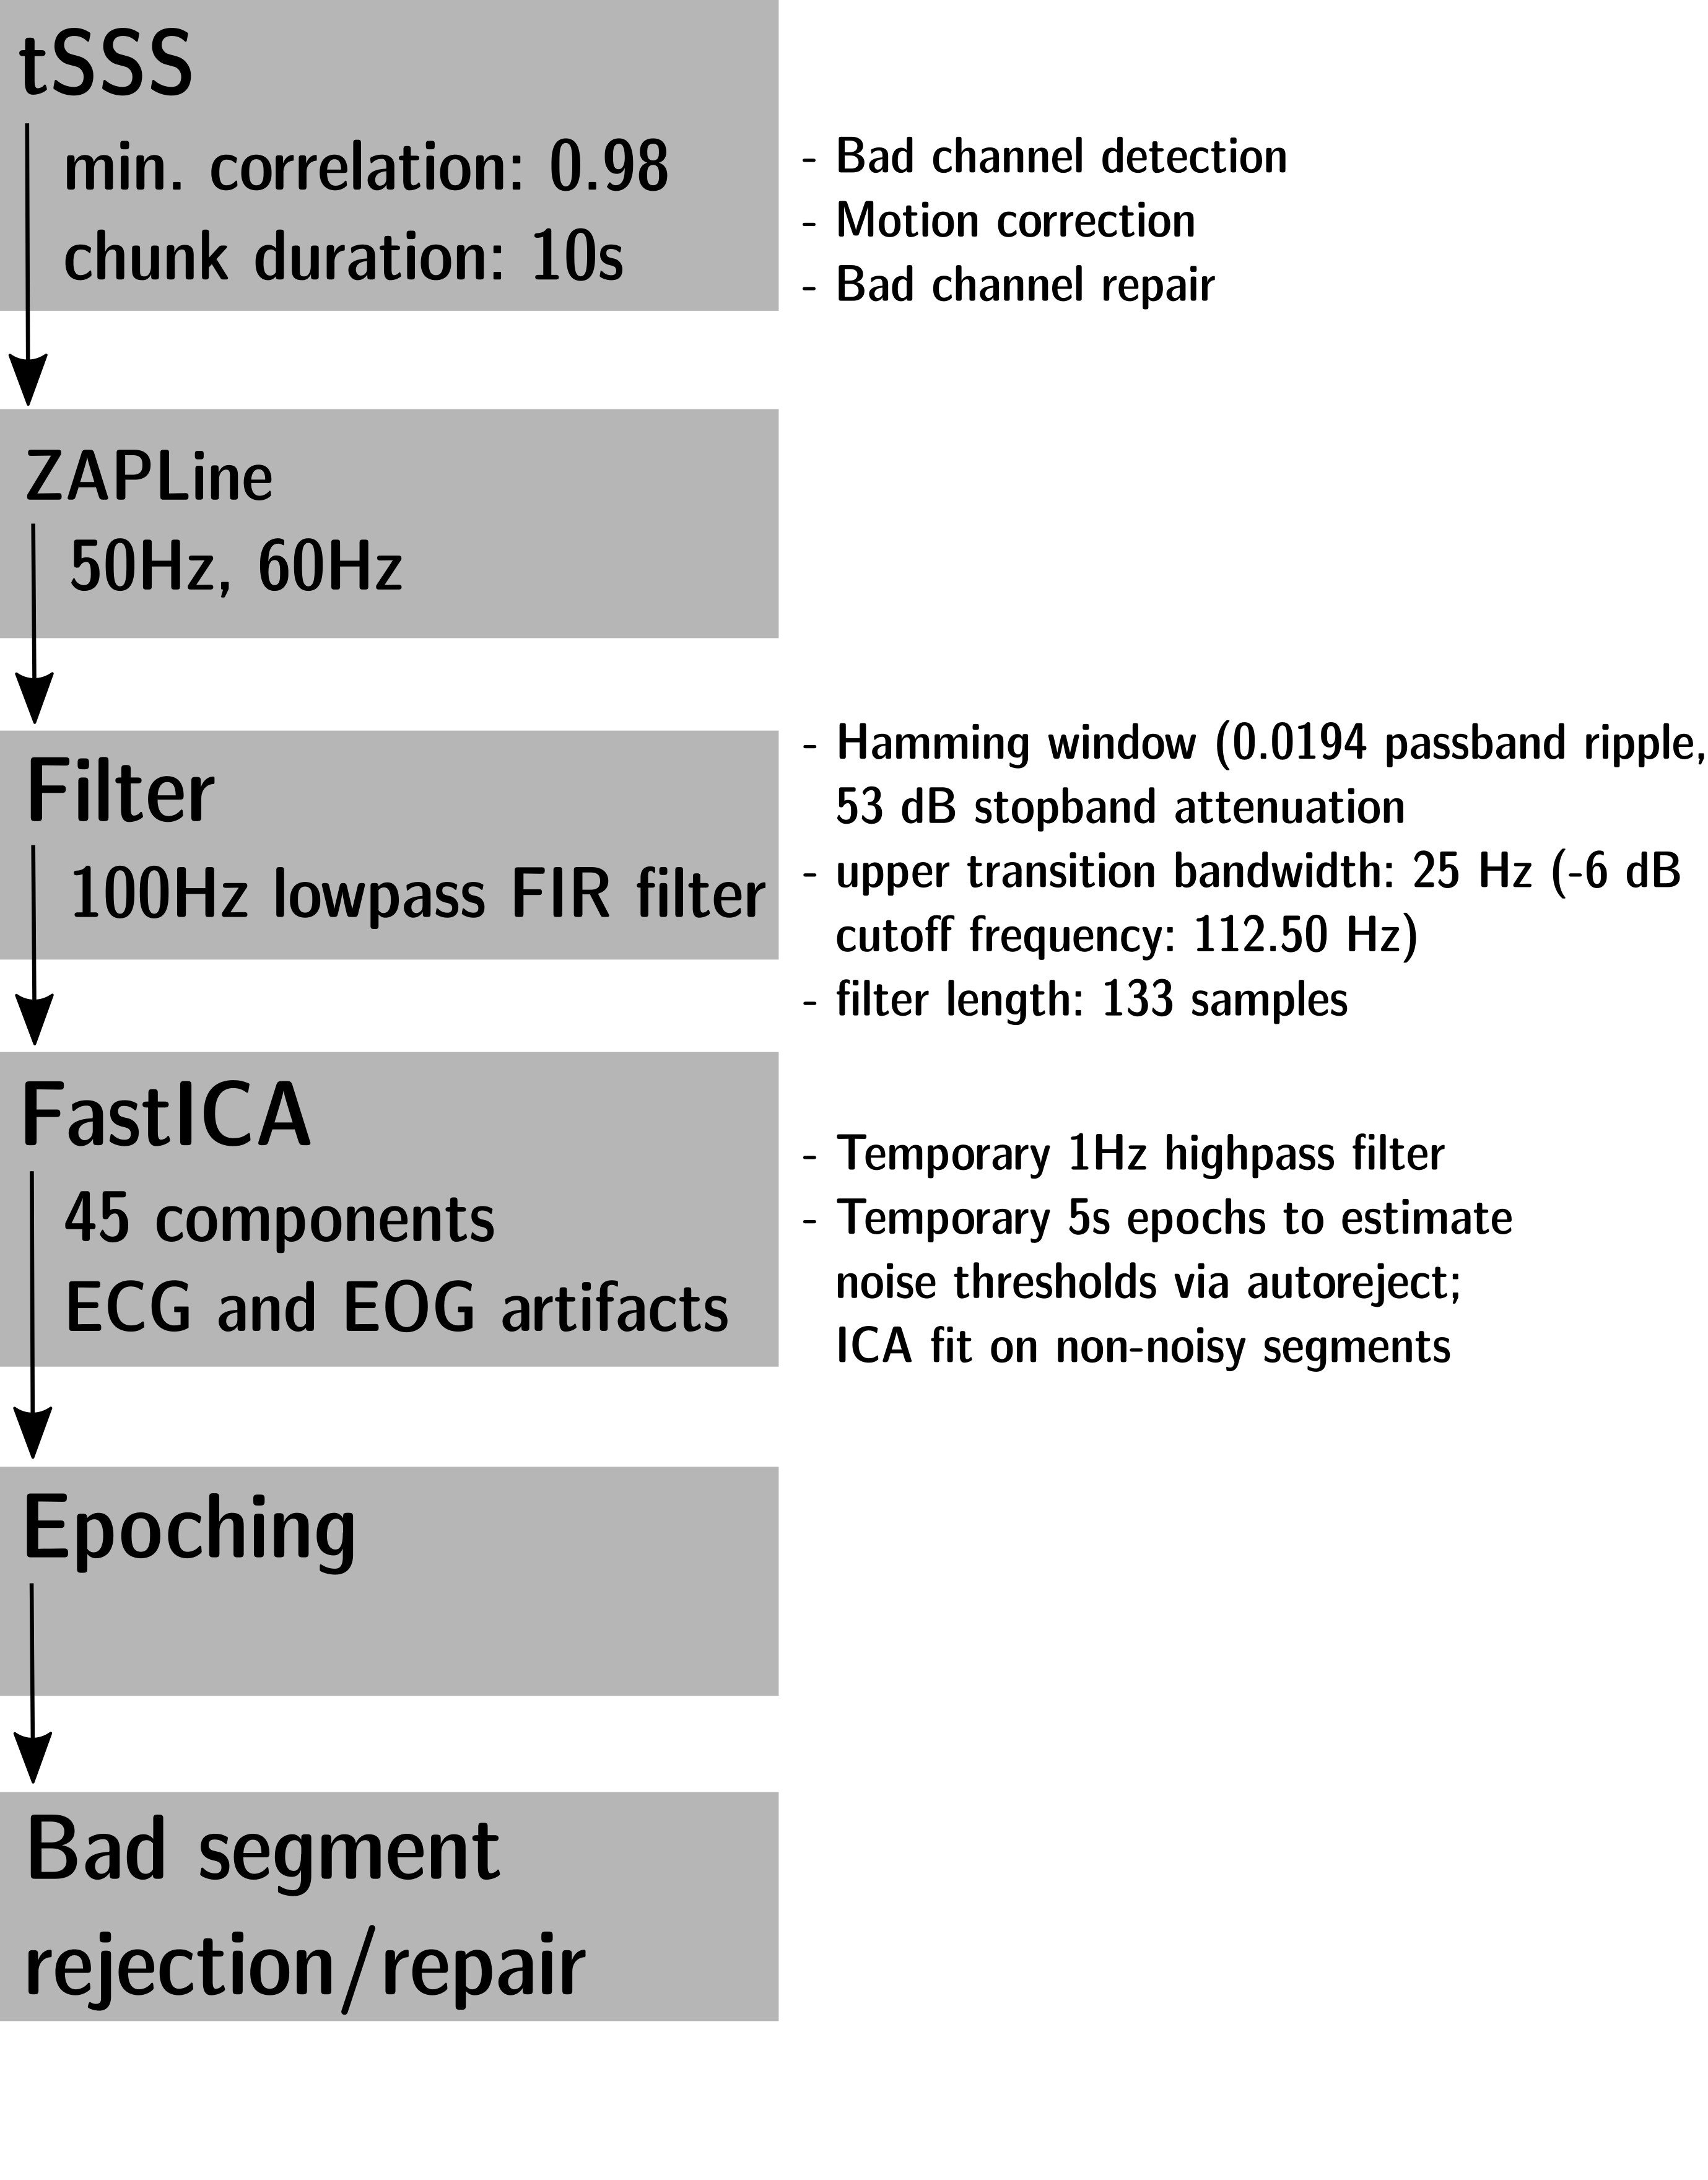
\includegraphics[width=\textwidth]{memento/preprocessing_overview.png}
		\caption[Preprocessing overview]{Preprocessing Overview}
		\label{fig:preproc}
	\end{subfigure}
	\begin{subfigure}{0.4\textwidth}
		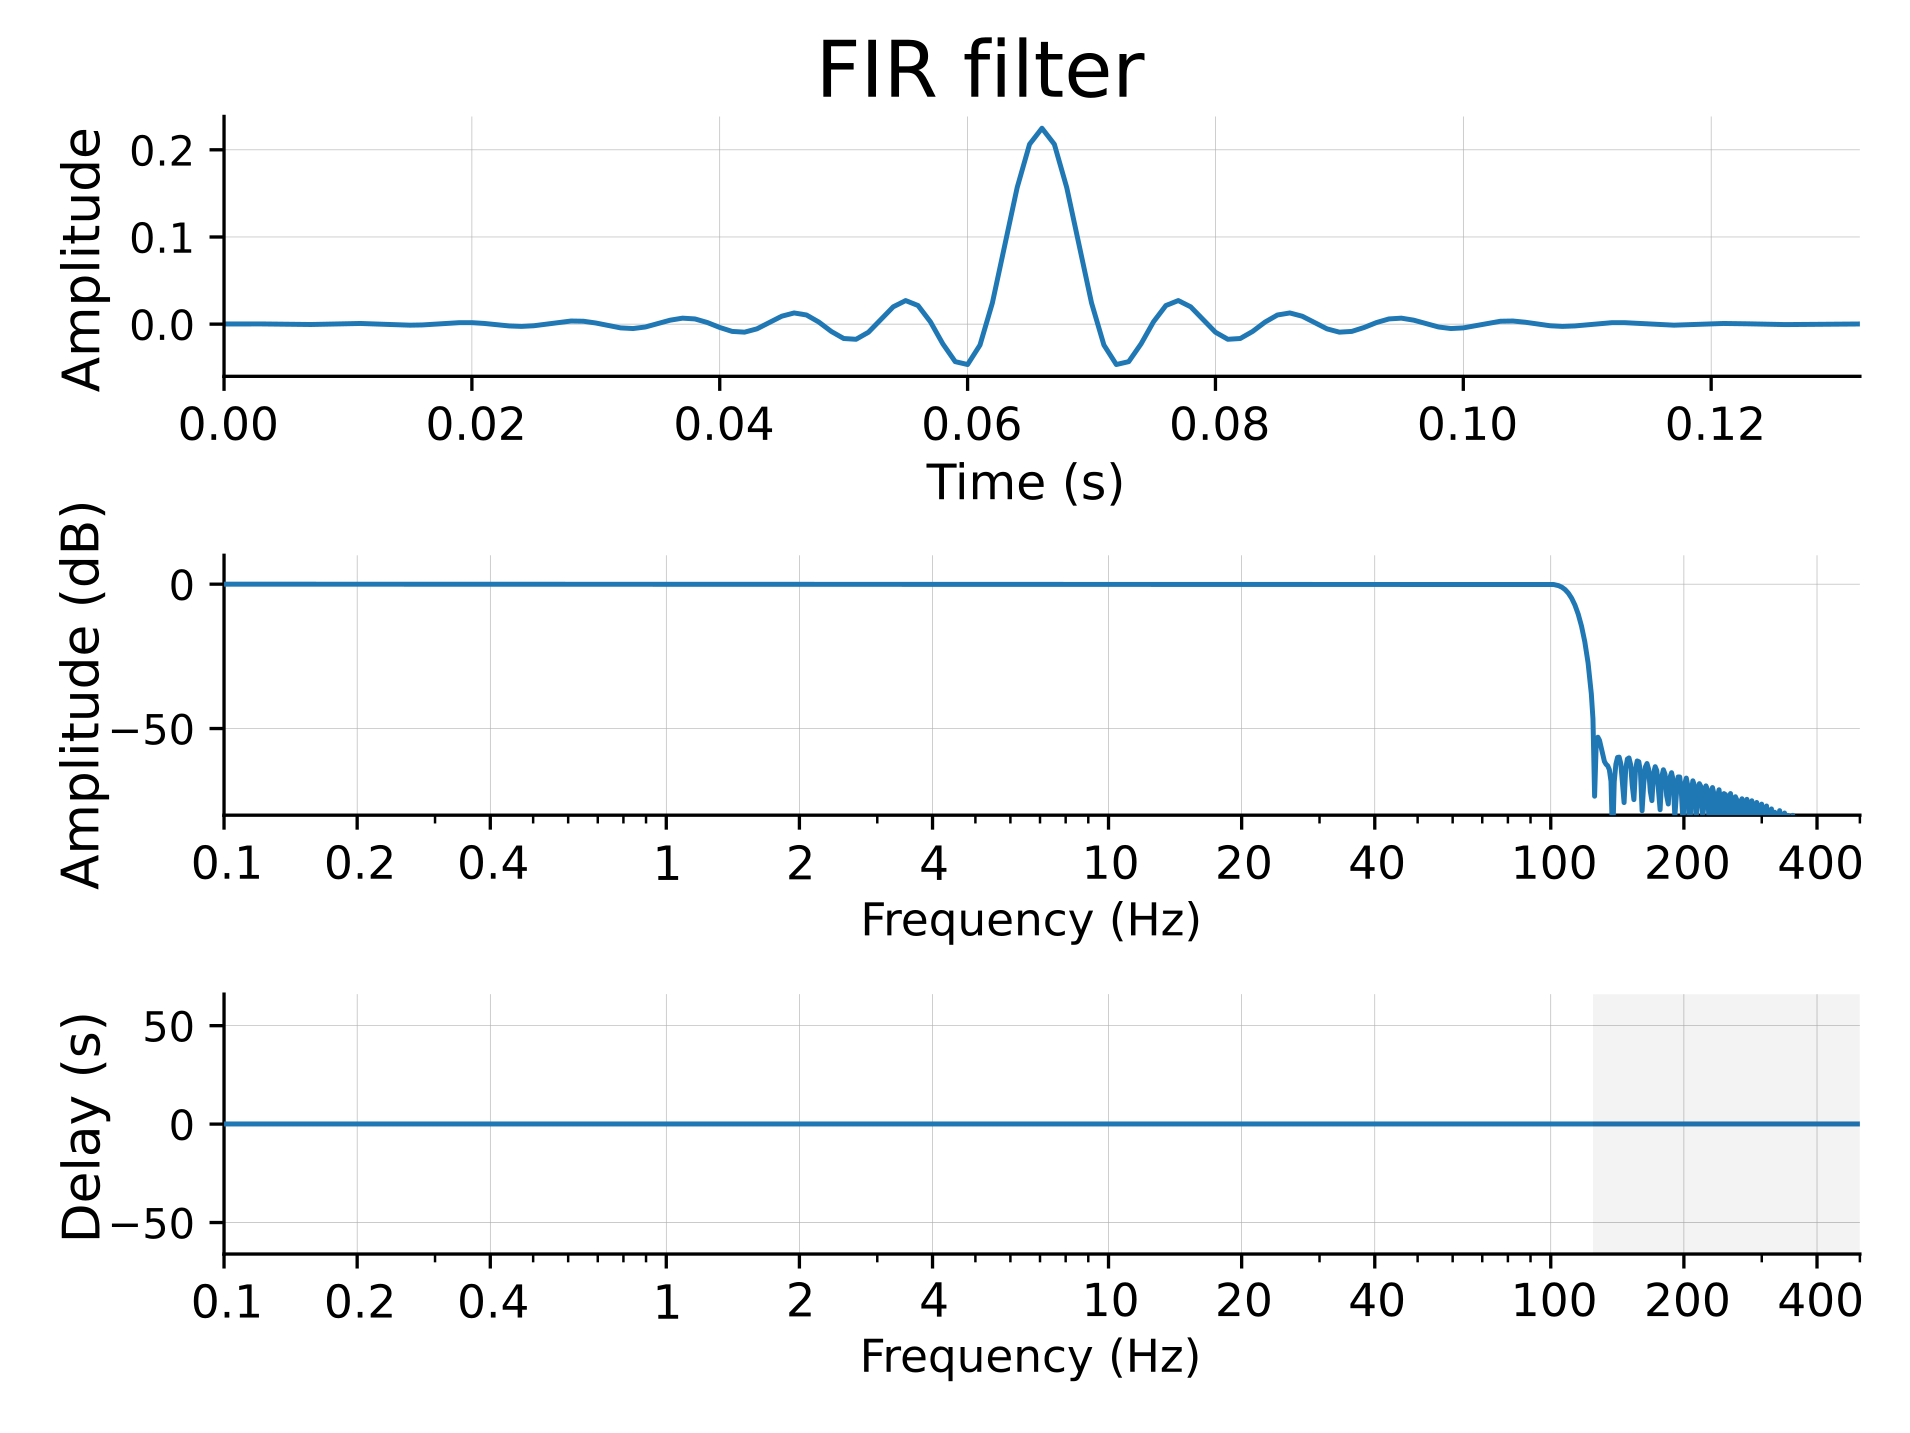
\includegraphics[width=\textwidth]{memento/filter_properties_100hz.png}
		\caption[Lowpass filter properties]{Lowpass filter properties}
		\label{fig:filter}
	\end{subfigure}
	\caption[Preprocessing]{Preprocessing thingies}
\end{figure}



Preprocessing consisted of the following sequential steps and is illustrated in Figure XX:
Temporal signal space separation (tsss) with movement corrections (TODO: retrieve parameters from the log files),
ZAPline filtering (CITE) to remove a ~60Hz spikes in the data, presumably from a presentation screen
Filtering (TODO: retrieve parameters from the log files)
Removal of heartbeat and eye blink artifacts with Independent component analysis (fastica)
Epoching into XXs without baseline correction. Bad epochs were interpolated or rejected using autoreject (CITE)

All preprocessing steps and the subsequent analysis were implemented using mne python (CITE) or custom Python functions. All preprocessing and analysis scripts are openly available on GitHub and as the python package \texttt{pymento\_meg} (CITE).


\pagebreak


\section{Simulation study}

MEG signal consists of oscillations with an amplitude, a frequency, and a phase.
Frequency, usually measured in hertz (Hz), is the number of times a specified event occurs within a specified time interval, while amplitude is the height, force or power of the wave, and power is the squared amplitude.
Phase involves the relationship between two or more signals that share the same frequency and describes the relationship between the position of the amplitude crests and troughs of two waveforms, measured in distance, time, or degrees.
If the peaks of two signals with the same frequency are in exact alignment at the same time, they are said to be in phase.
Conversely, if the peaks of two signals with the same frequency are not in exact alignment at the same time, they are said to be out of phase.
While shared response modeling, just like similar methods of hyper alignment [CITE], relies on the assumption that different participants display similar cognitive processes in response to the same tasks or stimuli [CITE], the exact timing or duration of such shared activity is subject to intra- and interindividual variation, and thus not necessarily phase-locked. [CITE]

[Link this to decision making tasks and previous methodological developments, such as Hidden Markov Models]

Spectral analysis consists of deconstructing a time domain signal of a given length into its constituent oscillatory components using Fourier analysis.
The resulting power spectrum displays a spectral decomposition, with the frequency domain of the oscillations on the x axis, and the amplitude on the y axis.
Thus, the signal is expressed as a function of frequency rather than time.
Such a transformation from a time-resolved representation of data to a representation in the frequency domain can be used to find shared signals with different temporal signatures [CITE probably every introductory MEG book].
Importantly, the transformations can be reversed using an inverse Fourier transform [CITE, add math].
In the context of shared response modeling we can make use of this reversibility by fitting the model on spectral data and then transforming the resulting shared space back into a time resolved space.
This not only allows the visualization of shared components as a time series but also easier interpretation of components in the context of the experimental paradigm.

A basic simulation illustrates the method:

Artificial signals, with parameters to change frequency, amplitude, length of the signal and length of the complete time series, can be generated.
\cref{fig:sim_artificial_signal} shows artificial examples, with 1000 samples of signal embedded in a time series of 10000 samples.
The main frequency component is 10Hz, with an amplitude of 1 and a varying amount of phase shift.

\begin{figure}
	\begin{subfigure}{1.0\textwidth}
		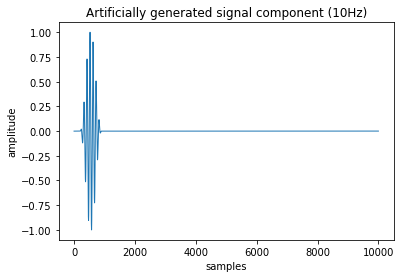
\includegraphics[width=.3\textwidth]{memento/simulation/sim_0.png}
		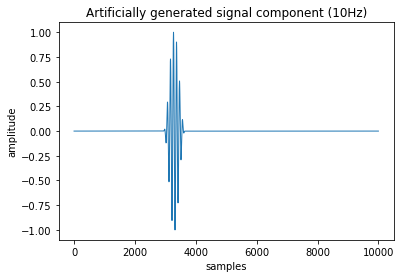
\includegraphics[width=.3\textwidth]{memento/simulation/sim_1.png}
		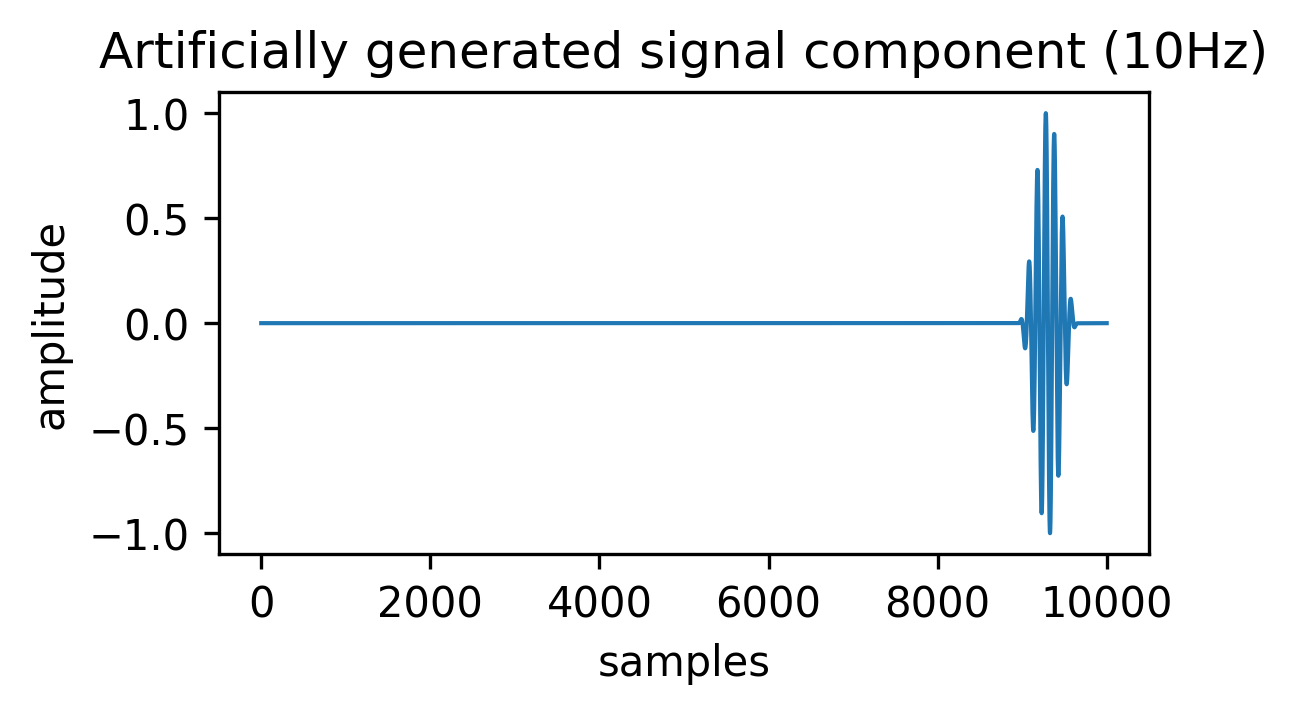
\includegraphics[width=.3\textwidth]{memento/simulation/sim_2.png}
		\label{fig:individualsignals}
		\caption{Three individual signals}
	\end{subfigure}
	\hfill
	\begin{subfigure}{0.4\textwidth}
		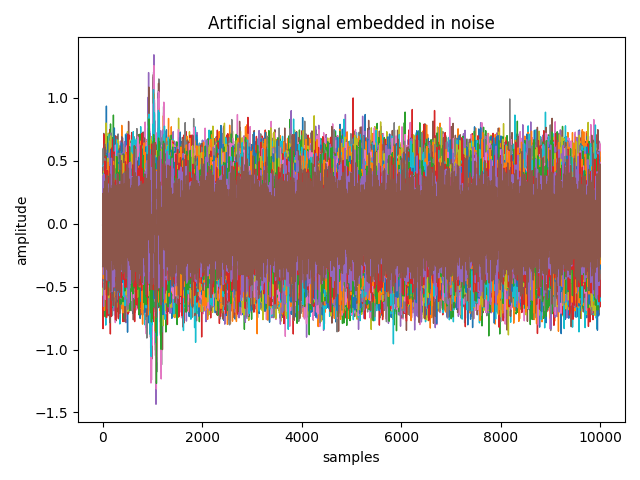
\includegraphics[width=\textwidth]{memento/simulation/sim_10.png}
		\label{fig:allsignals}
		\caption{signal in a subset of 306 sensors with Gaussian noise}
	\end{subfigure}
	\label{fig:sim_artificial_signal}
	\caption{Artificial signals with the same main frequency component, but different temporal offsets individually and combined.}
\end{figure}

We will use this signal as a ground truth signal to recover via SRM despite different phase shifts.
To simulate that it has been recorded with an MEG device, we add it to a 306-dimensional time series of random noise from 306 artificial sensors.
The signal is added to each sensors noise series with a sensor specific weight between 0 and 1, and a percentage specifying which percentage of sensors will contain some amount of signal.
Using this data as the basis for shared response modelling, we can fit a probabilistic shared response model with k=10 features in hopes to identify the signal as a shared component.
When this is done on time resolved data, the resulting shared space consists of components that differentially picked up signals from one or more participants, but represent it in a time series of repeated or overlapping signals that make an interpretation of individual components difficult (left).
The sensor weights that the model estimates for each component also do not show a clear association with the true weights used in the generation of the artificial data (right).

\begin{figure}
	\begin{subfigure}{.49\textwidth}
		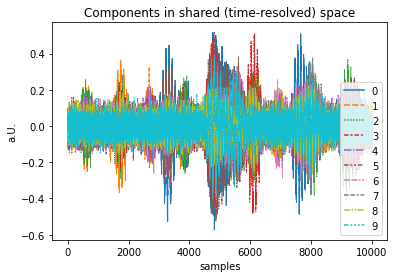
\includegraphics[width=\textwidth]{memento/simulation/sim_3.png}
	\end{subfigure}
	\begin{subfigure}{0.49\textwidth}
		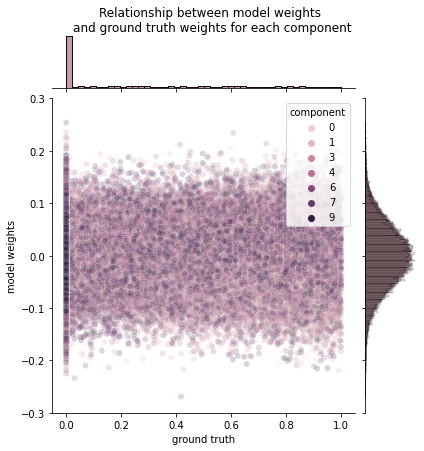
\includegraphics[width=\textwidth]{memento/simulation/sim_4.png}
	\end{subfigure}
	\label{fig:sim1}
	\caption{some caption}
\end{figure}

In other words, with phase shifts between individual simulations' signals, different components capture different participants' signals, but no general signal from the time-resolved and phase-shifted data. The relationship between model weights and ground truth weights appears mostly random.

However, transforming the signal into spectral space removes timing information.
While the components in spectral space are not easy to interpret or differentiate, the scatterplot reveal that certain components' weights show a clear association to the ground truth.


\begin{figure}
	\begin{subfigure}{.49\textwidth}
		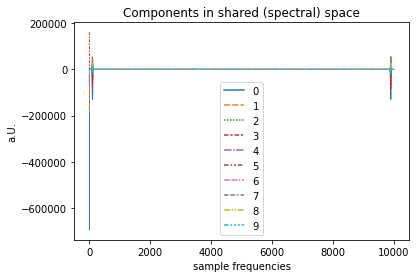
\includegraphics[width=\textwidth]{memento/simulation/sim_5.png}
	\end{subfigure}
	\begin{subfigure}{0.49\textwidth}
		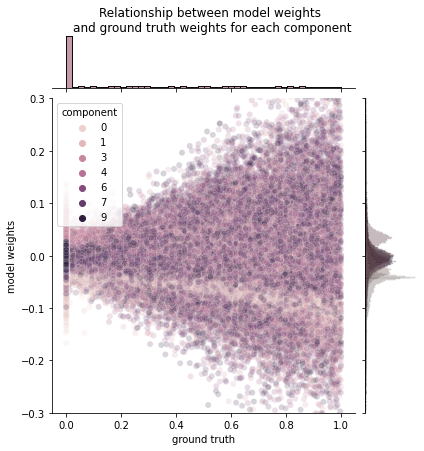
\includegraphics[width=\textwidth]{memento/simulation/sim_6.png}
	\end{subfigure}
	\label{fig:sim1}
	\caption{some caption}
\end{figure}

This becomes appearant when the raw data is transformed into the shared space by using the subject-specific weight matrices of the SRM model, and this subject-specific data is then transformed back from a spectral representation into a time-resolved representation via the inverse Fourier transform. One or few components are consistently representating the original signal well across subjects, laying the basis for both identifying shared signal in phase-shifted data and interpreting the shared components resulting from it.

\begin{figure}
	\begin{subfigure}{.3\textwidth}
		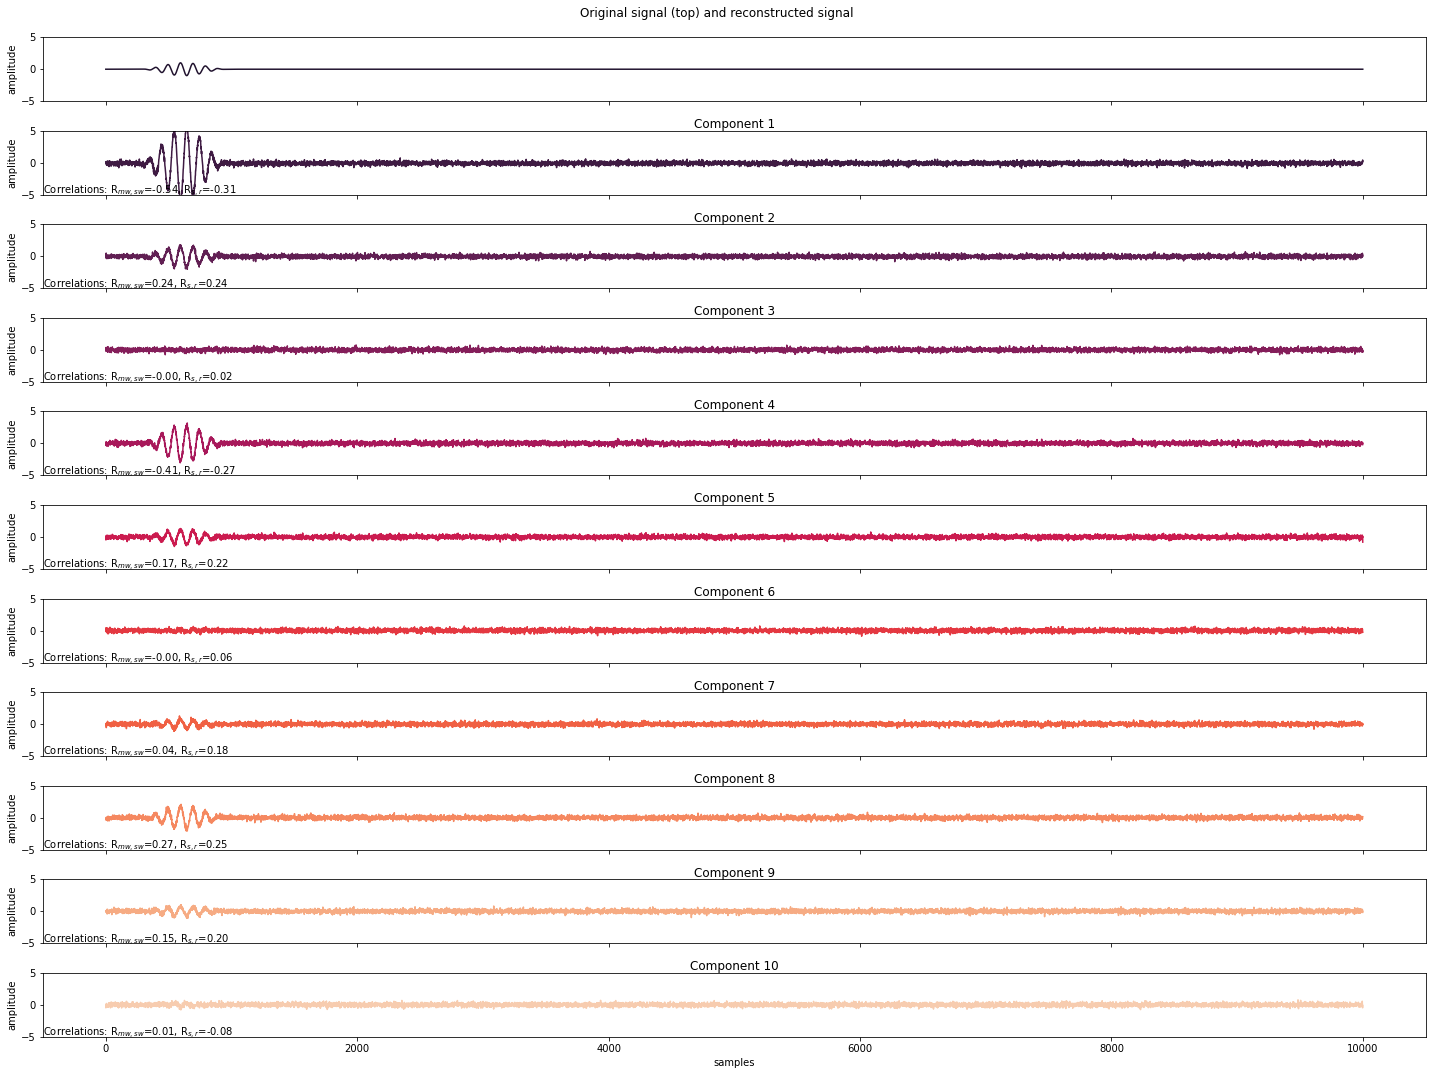
\includegraphics[width=\textwidth]{memento/simulation/sim_7.png}
	\end{subfigure}
	\begin{subfigure}{0.3\textwidth}
		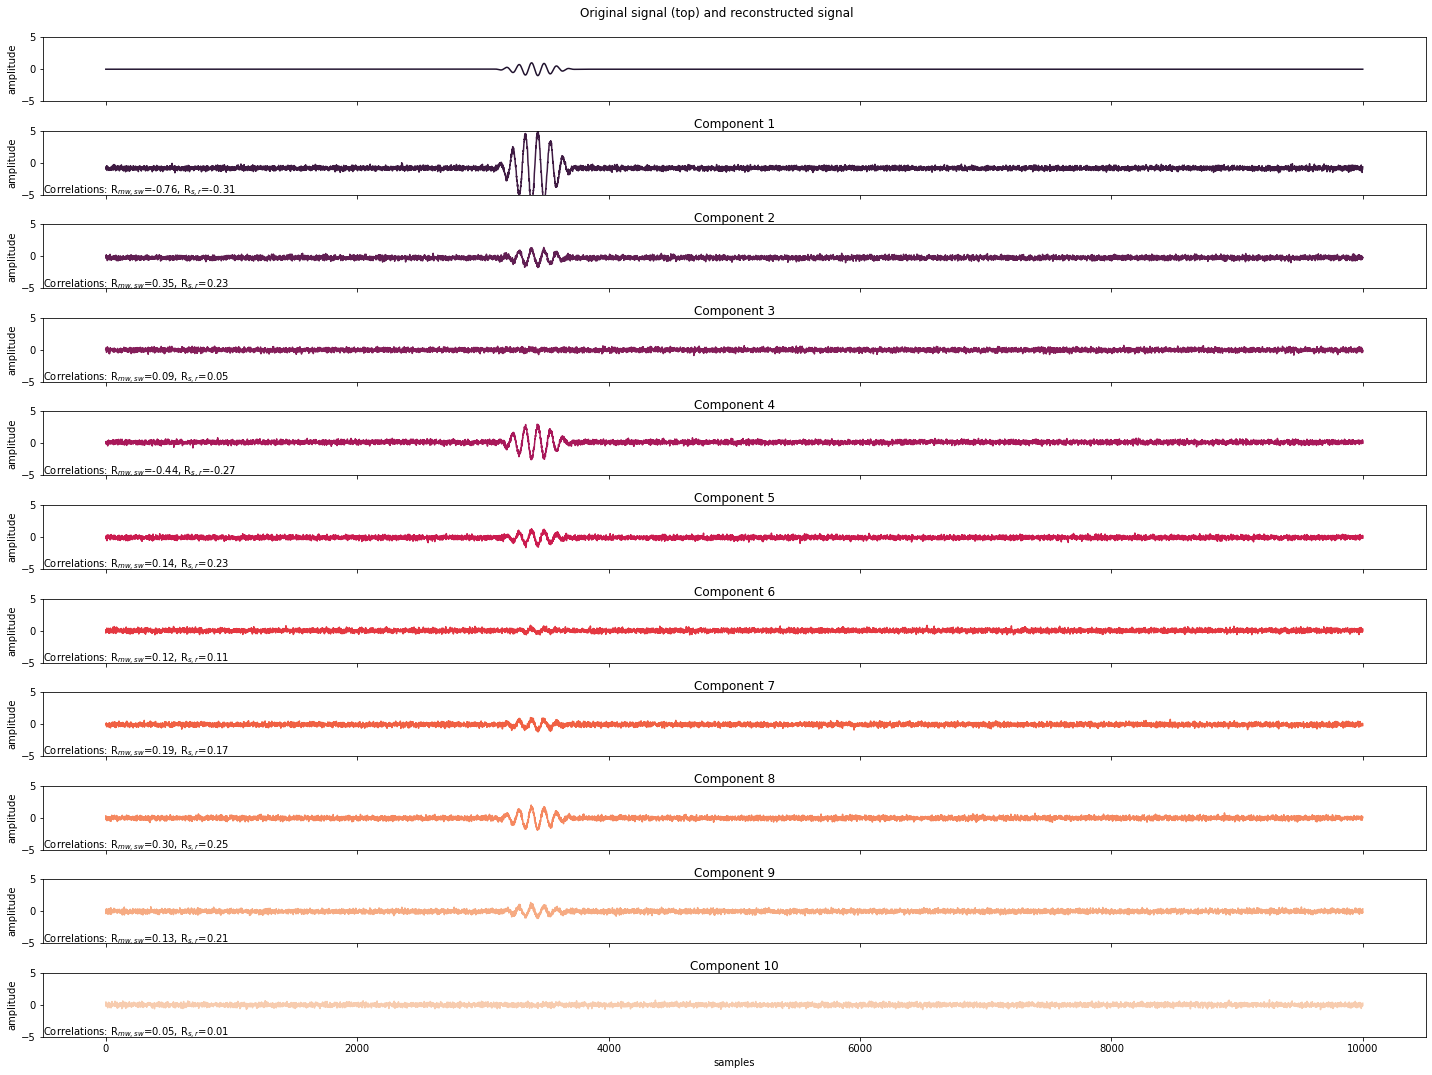
\includegraphics[width=\textwidth]{memento/simulation/sim_8.png}
	\end{subfigure}
	\begin{subfigure}{.3\textwidth}
		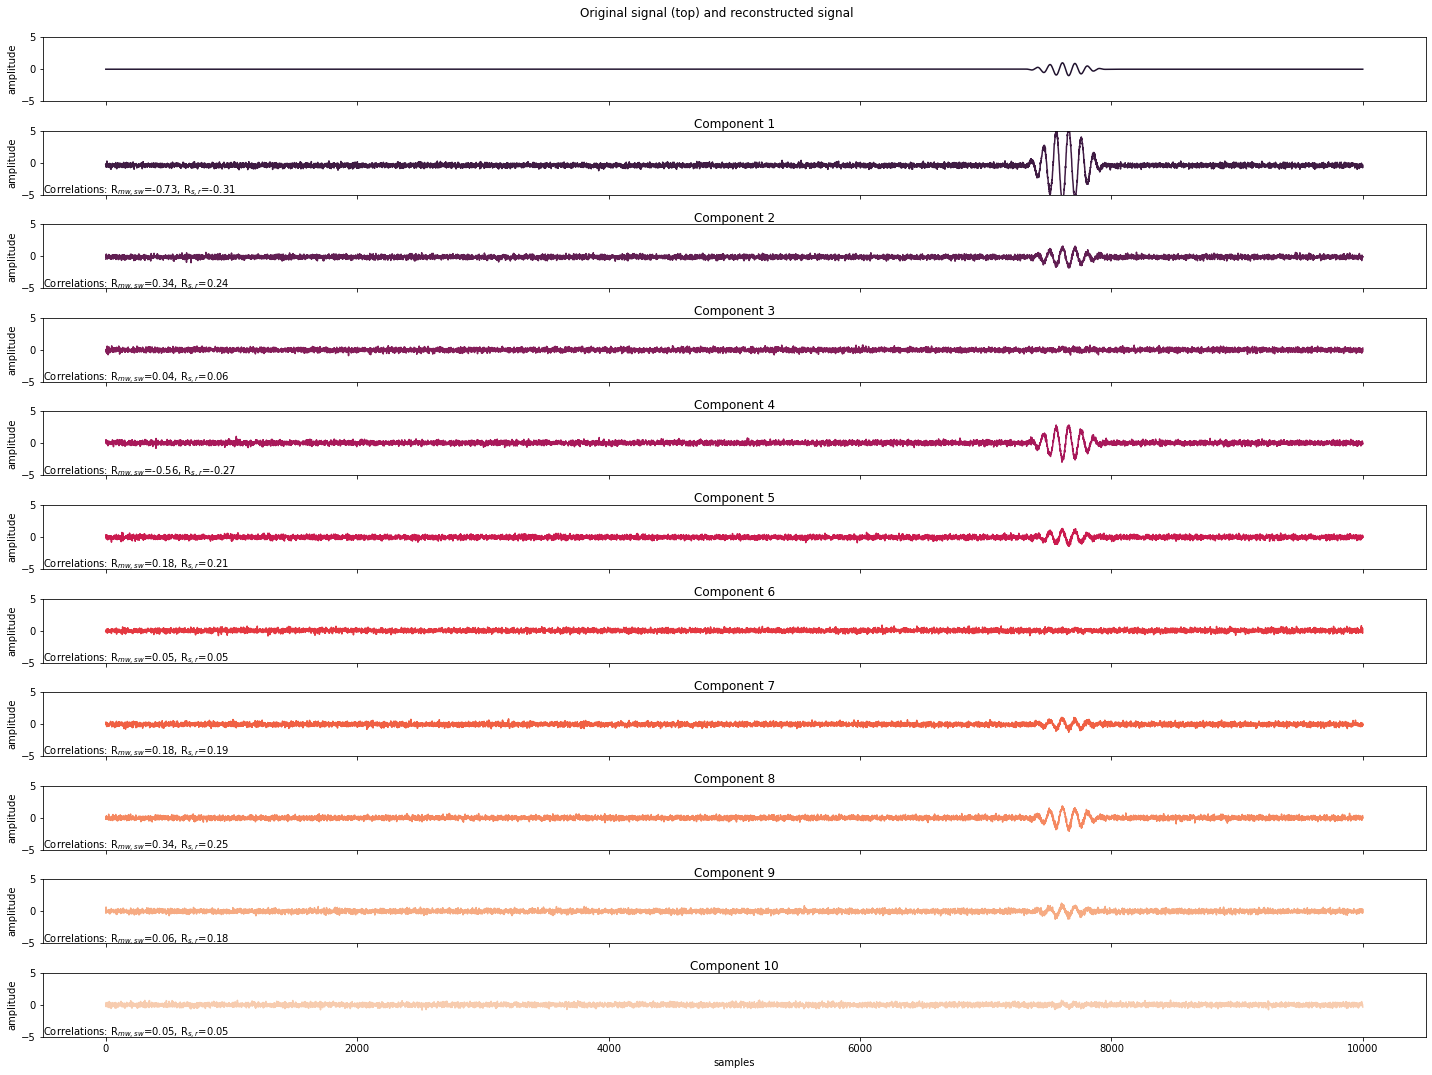
\includegraphics[width=\textwidth]{memento/simulation/sim_9.png}
	\end{subfigure}
	\label{fig:sim1}
	\caption{some caption}
\end{figure}

\pagebreak

\section{Temporal decoding}

From Grootswagers et al. (2017): MVPA for MEG/EEG
The term “multivariate pattern analysis” (or MVPA) en-
compasses a diverse set of methods for analyzing neuro-
imaging data. The common element that unites these
approaches is that they take into account the relation-
ships between multiple variables (e.g., voxels in fMRI or
channels in MEG/EEG), instead of treating them as inde-
pendent and measuring relative activation strengths. The
term “decoding” refers to the prediction of a model from
the data (“encoding” approaches do the reverse, predict-
ing the data from the model, reviewed in Naselaris, Kay,
Nishimoto, \& Gallant, 2011; see also, e.g., Ding \& Simon,
2012, for an example of encoding models for MEG). The
most common application of decoding in cognitive neu-
roscience is the use of machine learning classifiers (e.g.,
correlation classifiers (Haxby et al., 2001) or discriminant
classifiers (Carlson et al., 2003; Cox \& Savoy, 2003) to
identify patterns in neuroimaging data, which correspond
to the experimental task or stimulus. The most popular
applications of MVPA are decoding (for recent reviews on
fMRI decoding, see e.g., Haynes, 2015; Pereira et al., 2009)
and, more recently, representational similarity analysis
(RSA: Kriegeskorte \& Kievit, 2013).

\subsection{machine learning concepts in scikit-learn}

\texttt{y} is the \textit{target}, also called \texttt{outputs}, \texttt{responses}, \texttt{label} or \texttt{ground truth}.¸ Its the \texttt{dependent variable} in supervised learning, passed to an \texttt{estimator}'s fit method as y.
\texttt{X} is the observed data. Its number of rows are the number of \texttt{samples}.
\texttt{features} are the individual elements of a vector representing a sample. In a data matrix, features are represented as columns. Elsewhere features are also known as attributes, predictors, regressors, or independent variables.
\texttt{samples} typically denote a single feature vector. Elsewhere, a sample is called an instance, data point, or observation. \texttt{n\_samples} indicates the number of samples in a dataset, being the number of rows in a data array \texttt{X}


A \texttt{classifier} is a predictor with a finite set of discrete possible output values, and must implement "fit", "predict", and "score" methods, and could implement "decision\_function", "predict\_proba" and "predict\_log\_proba" methods.
An \texttt{estimator} is an object that manages the estimation and decoding of a model. An estimators fit method takes samples X, target y, and sample properties (e.g., weights). Once fitted, the "predict\_proba" method can return probability estimates for each class from some input data X. A \texttt{score} is a method that evaluates predictions on a given dataset, returning a single

\texttt{evaluation metrics} accept a ground truth and a prediction (e.g., output of predict, predict\_proba, etc)

\texttt{Transformers} (or \texttt{transforms}) can clean, reduce, expand, or generate feature representation.
 is
\texttt{Pipelines} sequentially chain transforms with a final estimator, and reduce the possibilities of forgetting transformations that could lead to inconsistent preprocessing applications between training and testing data and of leaking test data into training data. The purpose of a pipeline is to assemble several steps that can be cross-validated together whiule

\section{Results}
\pagebreak

